\documentclass[12pt,letterpaper]{article}
\usepackage{fullpage}
\usepackage[top=2cm, bottom=4.5cm, left=2.5cm, right=2.5cm]{geometry}
\usepackage{amsmath,amsthm,amsfonts,amssymb,amscd}
\usepackage{lastpage}
\usepackage{enumerate}
\usepackage{fancyhdr}
\usepackage{mathrsfs}
\usepackage{xcolor}
\usepackage{graphicx}
\usepackage{listings}
\usepackage{hyperref}
\usepackage{mathtools}

\hypersetup{%
  colorlinks=true,
  linkcolor=blue,
  linkbordercolor={0 0 1}
}
 



\lstdefinestyle{Python}{
    language        = Python,
    frame           = lines,
    basicstyle      = \footnotesize,
    keywordstyle    = \color{blue},
    stringstyle     = \color{green},
    commentstyle    = \color{red}\ttfamily
}

\setlength{\parindent}{0.0in}
\setlength{\parskip}{0.05in}

% Edit these as appropriate
\newcommand\sname{MIT2019066\\Koushal Kumar Sharma}

\newcommand \order{o}
\pagestyle{fancyplain}
\headheight 35pt
\lhead{SOC2020}
\rhead{\sname}
\chead{\textbf{\Large GA-ASSIGNMENT}}
\lfoot{}
\cfoot{}
\rfoot{\small\thepage}
\headsep 1.5em

\begin{document}
\textbf{\Large Answer: 1}\\\\
\textbf{Strings are :-}
\begin{itemize}
    \item $A_1$ = 11101111
    \item $A_2$ = 00010100
    \item $A_3$ = 01000011
\end{itemize}

\textbf{Schemata are :-}
\begin{itemize}
    \item $H_1$ = 1*******
    \item $H_2$ = 0*******
    \item $H_3$ = ******11
    \item $H_4$ = ***0*01*
    \item $H_5$ = 1*****1*
\end{itemize}
\textbf{\large Schemata and String matching :-}
\begin{itemize}
    \item $H_1$ = $A_1$
    \item $H_2$ = $A_2, A_3$
    \item $H_3$ = $A_1, A_3$
    \item $H_4$ = $A_3$
    \item $H_5$ = $A_1$
\end{itemize}

\textbf{\large Order and Length of Schemata :-}
$\delta(H)$ is length, and $\order(H)$ is Order.
\begin{itemize}
    \item $H_1$ = $\delta(H_1) = 0$, $\order(H_1) = 1$
    \item $H_2$ = $\delta(H_2) = 0$, $\order(H_2) = 1$
    \item $H_3$ = $\delta(H_3) = 1$, $\order(H_3) = 2$
    \item $H_4$ = $\delta(H_4) = 3$, $\order(H_4) = 3$
    \item $H_5$ = $\delta(H_5) = 6$, $\order(H_5) = 2$\\
\end{itemize}

\textbf{\large Survival of each Schemata under Mutation :-}\\\\
Probability of single mutation is $p_m = 0.001$
For a schema H to survive, all fixed bits must remain unchanged.\\
\\The probability of a schema H survives under mutation is
\begin{equation}
    S_m(H) = (1 - p_m) ^ {\order(H)}
\end{equation}
We can rewrite according to given $p_m$ is 
$$S_m(H) = (1 - 0.001)^ {\order(H)}$$
$$S_m(H) = (0.999)^ {\order(H)}$$
Taking $\order(H)$ of schemeta from above calculated.
\begin{itemize}
    \item $S_m(H_1)$ = $(0.999)^ {1}$ = $0.999$
    \item $S_m(H_2)$ = $(0.999)^ {1}$ = $0.999$
    \item $S_m(H_3)$ = $(0.999)^ {2}$ = $0.998$
    \item $S_m(H_4)$ = $(0.999)^ {3}$ = $0.997$
    \item $S_m(H_5)$ = $(0.999)^ {2}$ = $0.998$
\end{itemize}

\textbf{\large Survival of each Schemata under Cross Over :-}\\\\
Probability of Crossover = $p_c = 0.85$
\\The probability of a schema H survives under cross over is
\begin{equation}
    S_c(H) \geqslant 1 - p_c \frac{\delta(H)}{l - 1}
\end{equation}
as l = 8, we can rewrite this as
$$S_c(H) \geqslant 1 - (0.85) \frac{\delta(H)}{7}$$
Taking $\delta(H)$ of schemeta from above calculated.
\begin{itemize}
    \item $S_c(H_1) \geqslant 1 - (0.85) \frac{0}{7} = 1$
    \item $S_c(H_2) \geqslant 1 - (0.85) \frac{0}{7} = 1$
    \item $S_c(H_3) \geqslant 1 - (0.85) \frac{1}{7} = 0.878$
    \item $S_c(H_4) \geqslant 1 - (0.85) \frac{3}{7} = 0.635$
    \item $S_c(H_5) \geqslant 1 - (0.85) \frac{6}{7} = 0.271$
\end{itemize}

\newpage
\textbf{\Large Answer: 2}\\\\
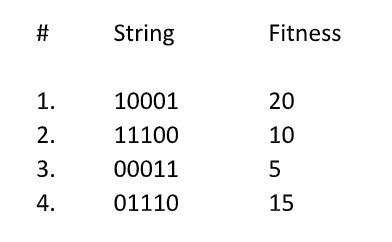
\includegraphics[]{a}

\textbf{Schemata are} :- 
\begin{center}
    $H_1$ = 1****\\
    $H_2$ = 0**1*\\
\end{center}
$p_m = 0.01$\\
$p_c = 0.7$\\

\textbf{Expectation of Schema H in Next Generation is:-}
\begin{equation}
    E[m(H, k+1)] \geqslant m(H,k) \frac{f(H,k)}{\bar{f}} (1 - p_c \frac{\delta(H)}{l - 1}) (1 - p_m)^{\order(H)}
\end{equation}
Where :-
$$m(H,k)\text{ = denotes the number of instances of H in the k-th generation}$$
$$f(H,k)\text{ = denotes average fitness of H in the k-th generation}$$
$$\bar{f}\text{ = denotes avergae fitness of population in k-th generation}$$\\

\textbf{Expected number of Schema $H_1$ in generation 1 :-}\\
$$H_1 = \text{1****}$$
$$k+1 = 1, k = 0$$
There are two string 1 and 2 belongs to schema $H_1$, and there fitness are 20 and 10
$$m(H_1,0) = 2$$
$$f(H_1,0) = (20+10)/2 = 15$$
$$\bar{f} = 50/4$$
$$ l = 5$$
$$\delta(H_1) = 0$$
$$\order(H_1) = 1$$
Using equation 3 for calculation of expectation and putting corresponding values :-

$$ E[m(H_1,1)] \geqslant 2 * \frac{15}{50/4} * (1 - 0.7 * \frac{0}{4}) (1 - 0.01)^1$$


\begin{center}
    \boxed{$$ E[m(H_1,1)] \geqslant 2.376$$}
\end{center}

\textbf{\\}

\textbf{Expected number of Schema $H_2$ in generation 1 :-}\\
$$H_2 = \text{0**1*}$$
$$k+1 = 1, k = 0$$
There are two string 3 and 4 belongs to schema $H_2$, and there fitness are 5 and 15
$$m(H_2,0) = 2$$
$$f(H_2,0) = (5+15)/2 = 10$$
$$\bar{f} = 50/4$$
$$ l = 5$$
$$\delta(H_2) = 3$$
$$\order(H_2) = 2$$
Using equation 3 for calculation of expectation and putting corresponding values :-

$$ E[m(H_2,1)] \geqslant 2 * \frac{10}{50/4} * (1 - 0.7 * \frac{3}{4}) (1 - 0.01)^2$$

\begin{center}
    \boxed{$$ E[m(H_2,1)] \geqslant 0.744$$}
\end{center}
\end{document}
putting